\documentclass[11pt,a4paper]{article}

\usepackage[margin=2.2cm]{geometry}
\usepackage{amsmath,amssymb,amsthm}
\usepackage{booktabs}
\usepackage{array}
\usepackage{tabularx}
\usepackage[shortlabels]{enumitem}
\usepackage{xcolor}
\usepackage{tikz}
\usepackage{fancyhdr}
\usepackage{setspace}
\usepackage{microtype}
\usepackage{titlesec}
\usepackage{hyperref}
\usepackage{listings}
\usepackage[skins,breakable]{tcolorbox}

\usetikzlibrary{positioning,arrows.meta,calc,fit,shapes.geometric,matrix,decorations.pathreplacing}

\definecolor{ink}{HTML}{222222}
\definecolor{rulegray}{HTML}{444444}
\definecolor{boxline}{HTML}{666666}
\definecolor{boxfill}{HTML}{F4F4F4}
\definecolor{boxtitle}{HTML}{E8E8E8}
\definecolor{g1}{HTML}{D0D0D0}
\definecolor{g2}{HTML}{9A9A9A}
\definecolor{g3}{HTML}{5A5A5A}

\hypersetup{
  colorlinks=true,
  linkcolor=black,
  urlcolor=black,
  pdftitle={MTL 458 Lecture 20: Concurrency Bugs},
  pdfauthor={Minati De, IIT Delhi}
}

\setstretch{1.12}
\raggedbottom
\setlist[itemize]{leftmargin=1.3em,itemsep=0.28em,topsep=0.35em}
\setlist[enumerate]{leftmargin=1.5em,itemsep=0.35em,topsep=0.4em}

\titleformat{\section}
  {\Large\bfseries\color{ink}}{\thesection.}{0.6em}{}
  [{\color{rulegray}\titlerule[0.5pt]}]
\titleformat{\subsection}
  {\large\bfseries\color{ink}}{\thesubsection}{0.55em}{}
\titleformat{\subsubsection}
  {\normalsize\bfseries\color{ink}}{\thesubsubsection}{0.5em}{}

\titlespacing*{\section}{0pt}{1.35em}{0.7em}
\titlespacing*{\subsection}{0pt}{1.05em}{0.45em}

\pagestyle{fancy}
\fancyhf{}
\renewcommand{\headrulewidth}{0.4pt}
\renewcommand{\footrulewidth}{0.3pt}
\fancyhead[L]{\small\color{ink}MTL 458 \textbullet\ Operating Systems}
\fancyhead[R]{\small\color{ink}Lecture 20: Concurrency Bugs}
\fancyfoot[C]{\small\thepage}
\setlength{\headheight}{14pt}

% ---------------------------------------------------------------------------
% Boxes
% ---------------------------------------------------------------------------
\tcbset{
  commonbox/.style={
    colback=boxfill, colframe=boxline, boxrule=0.5pt,
    left=6pt, right=6pt, top=5pt, bottom=5pt,
    fonttitle=\bfseries, coltitle=black, colbacktitle=boxtitle,
    enhanced, sharp corners=south, breakable
  }
}
\newtcolorbox{keybox}[1][]{commonbox, title={#1}}
\newtcolorbox{quizbox}[1][]{commonbox, title={#1}}
\newtcolorbox{solbox}[1][]{commonbox, title={#1}}
\newtcolorbox{warnbox}[1][]{commonbox, title={#1}}
\newtcolorbox{defbox}[1][]{commonbox, title={#1}}

\lstset{
  language=C,
  basicstyle=\ttfamily\small,
  keywordstyle=\bfseries,
  commentstyle=\itshape\color{g3},
  numbers=left, numberstyle=\scriptsize\color{g2}, numbersep=6pt,
  frame=single, rulecolor=\color{boxline},
  backgroundcolor=\color{boxfill},
  xleftmargin=1.6em, framexleftmargin=1.4em,
  columns=fullflexible, keepspaces=true,
  showstringspaces=false, breaklines=true,
  aboveskip=0.6em, belowskip=0.6em,
  morekeywords={set_t,node_t,pthread_mutex_t,pthread_cond_t}
}

% Start a new page unless at least #1 of vertical space remains
\makeatletter
\newcommand{\keepspace}[1]{\par\penalty-100\begingroup
  \setlength{\dimen@}{#1}\dimen@ii\pagegoal\advance\dimen@ii-\pagetotal
  \ifdim\dimen@>\dimen@ii\ifdim\dimen@ii>\z@\vfil\fi\break\fi\endgroup}
\makeatother

% ---------------------------------------------------------------------------
% Four-way-stop intersection: \crossing{car list}{caption}
% car list entries: x/y/label/orientation(h or v)/shade
% ---------------------------------------------------------------------------
\newcommand{\crossing}[2]{%
\begin{tikzpicture}[x=0.78cm, y=0.78cm,
    stop/.style={regular polygon, regular polygon sides=8, fill=black!70,
      inner sep=0pt, minimum size=0.2cm}]
  \fill[black!6] (-3,-2.4) rectangle (3,2.4);
  \fill[g1] (-3,-0.5) rectangle (3,0.5);
  \fill[g1] (-0.5,-2.4) rectangle (0.5,2.4);
  \foreach \x in {-2.8,-2.0,-1.2, 0.8,1.6,2.4} \draw[line width=1pt, white] (\x,0) -- ++(0.4,0);
  \foreach \y in {-2.2,-1.4, 0.8,1.6} \draw[line width=1pt, white] (0,\y) -- ++(0,0.4);
  \foreach \p in {(-0.72,0.72),(0.72,0.72),(-0.72,-0.72),(0.72,-0.72)} \node[stop] at \p {};
  \foreach \x/\y/\l/\ori/\shade in {#1} {
    \if\ori h
      \node[draw, fill=\shade, minimum width=0.6cm, minimum height=0.22cm, inner sep=0pt,
            font=\tiny\bfseries, text=white] at (\x,\y) {\l};
    \else
      \node[draw, fill=\shade, minimum width=0.22cm, minimum height=0.6cm, inner sep=0pt,
            font=\tiny\bfseries, text=white] at (\x,\y) {\l};
    \fi
  }
  \node[font=\scriptsize, align=center] at (0,-2.85) {#2};
\end{tikzpicture}}

\begin{document}

% ===========================================================================
% Title
% ===========================================================================
\begin{center}
{\small\itshape Made by Arpit's Milo}\\[0.3em]
{\color{rulegray}\rule{\textwidth}{1.1pt}}\\[0.45em]
{\LARGE\bfseries Operating Systems}\\[0.25em]
{\Large\bfseries MTL 458 \textperiodcentered\ Lecture 20}\\[0.35em]
{\LARGE\bfseries Concurrency Bugs}\\[0.35em]
{\large Minati De}\\[0.15em]
{\normalsize Department of Mathematics, Indian Institute of Technology Delhi}\\[0.35em]
{\color{rulegray}\rule{\textwidth}{1.1pt}}
\end{center}

\vspace{0.4em}
\begin{keybox}[Questions answered in this lecture]
\begin{itemize}
  \item Why is concurrent programming difficult?
  \item What type of concurrency bugs occur?
  \item How to fix \textbf{atomicity bugs} (with locks)?
  \item How to fix \textbf{ordering bugs} (with condition variables)?
  \item How does \textbf{deadlock} occur?
  \item How to prevent deadlock (with \textbf{wait-free algorithms}, \textbf{grab
        all locks atomically}, \textbf{trylocks}, and \textbf{ordering across
        locks})?
\end{itemize}
\end{keybox}

\tableofcontents
\vspace{0.6em}
\noindent{\color{rulegray}\rule{\textwidth}{0.4pt}}

% ===========================================================================
\section{Why concurrency bugs matter}
% ===========================================================================

\subsection{Concurrency in medicine: Therac-25 (1980's)}

Therac-25 was a radiation-therapy machine. A software race condition in it
killed patients:

\begin{quote}
\itshape ``The accidents occurred when the high-power electron beam was
activated instead of the intended low power beam, and without the beam
spreader plate rotated into place. Previous models had hardware interlocks in
place to prevent this, but Therac-25 had removed them, depending instead on
software interlocks for safety. The software interlock could fail due to a
\textbf{race condition}.''

``\ldots in three cases, the injured patients \textbf{later died}.''
\end{quote}
\noindent{\small Source: \url{http://en.wikipedia.org/wiki/Therac-25}}

\subsection{Concurrency study from 2008 (Lu et al.)}

\textbf{Lu et al.\ study:} for four major projects, search for concurrency
bugs among \(>\)500K bug reports. Analyze a small sample to identify common
types of concurrency bugs.
{\small (Source: \url{http://pages.cs.wisc.edu/~shanlu/paper/asplos122-lu.pdf})}

\begin{center}
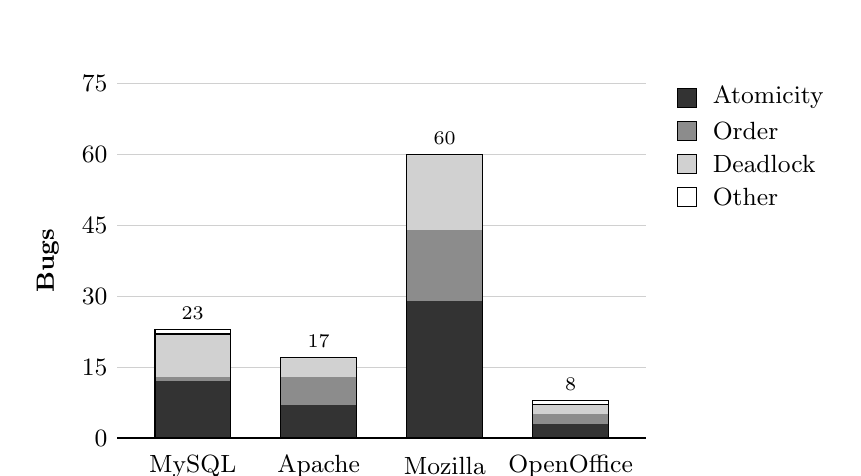
\begin{tikzpicture}[x=1.6cm, y=0.06cm]
  % axes and grid
  \foreach \v in {0,15,30,45,60,75} {
    \draw[g1] (0.4,\v) -- (4.6,\v);
    \node[anchor=east, font=\small] at (0.4,\v) {\v};
  }
  \draw[thick] (0.4,0) -- (4.6,0);
  \node[rotate=90, font=\small\bfseries] at (-0.15,37.5) {Bugs};
  % stacked bars: Atomicity, Order, Deadlock, Other
  \foreach \i/\name/\a/\o/\d/\t in {1/MySQL/12/1/9/1, 2/Apache/7/6/4/0,
                                    3/Mozilla/29/15/16/0, 4/OpenOffice/3/2/2/1} {
    \pgfmathsetmacro{\yo}{\a}
    \pgfmathsetmacro{\yd}{\a+\o}
    \pgfmathsetmacro{\yt}{\a+\o+\d}
    \pgfmathsetmacro{\ye}{\a+\o+\d+\t}
    \fill[black!80] (\i-0.3,0) rectangle (\i+0.3,\yo);
    \fill[black!45] (\i-0.3,\yo) rectangle (\i+0.3,\yd);
    \fill[black!18] (\i-0.3,\yd) rectangle (\i+0.3,\yt);
    \draw[fill=white] (\i-0.3,\yt) rectangle (\i+0.3,\ye);
    \draw (\i-0.3,0) rectangle (\i+0.3,\ye);
    \node[font=\small] at (\i,-6) {\name};
    \node[font=\scriptsize, above] at (\i,\ye) {\pgfmathprintnumber{\ye}};
  }
  % legend
  \foreach \k/\c/\l in {0/black!80/Atomicity, 1/black!45/Order, 2/black!18/Deadlock, 3/white/Other} {
    \draw[fill=\c] (4.85,70-\k*7) rectangle ++(0.15,4);
    \node[anchor=west, font=\small] at (5.05,72-\k*7) {\l};
  }
\end{tikzpicture}
\end{center}

\begin{center}
\small
\renewcommand{\arraystretch}{1.15}
\begin{tabular}{@{}lccccc@{}}
  \toprule
  \textbf{Project} & \textbf{Atomicity} & \textbf{Order} & \textbf{Deadlock} & \textbf{Other} & \textbf{Total} \\
  \midrule
  MySQL      & 12 & 1  & 9  & 1 & 23 \\
  Apache     & 7  & 6  & 4  & 0 & 17 \\
  Mozilla    & 29 & 15 & 16 & 0 & 60 \\
  OpenOffice & 3  & 2  & 2  & 1 & 8 \\
  \midrule
  \textbf{Total} & 51 & 24 & 31 & 2 & 108 \\
  \bottomrule
\end{tabular}

{\small (Values are the chart's data in the slides; the totals are added
here.)}
\end{center}

The lecture returns to this chart three times, once for each of the three big
categories: \textbf{atomicity} bugs (Section~\ref{sec:atom}), \textbf{order}
bugs (Section~\ref{sec:order}) and \textbf{deadlock} (Section~\ref{sec:dl}).
Atomicity and order bugs are the two \emph{non-deadlock} kinds, and together
they make up most of the bugs found.

% ===========================================================================
\section{Atomicity bugs}\label{sec:atom}
% ===========================================================================

\subsection{Example: MySQL}

\begin{center}
\begin{minipage}[t]{0.5\textwidth}
\textbf{Thread 1:}
\begin{lstlisting}[numbers=none]
if (thd->proc_info) {
    ...
    fputs(thd->proc_info, ...);
    ...
}
\end{lstlisting}
\end{minipage}\hfill
\begin{minipage}[t]{0.44\textwidth}
\textbf{Thread 2:}
\begin{lstlisting}[numbers=none]
thd->proc_info = NULL;
\end{lstlisting}
\end{minipage}
\end{center}

\begin{quizbox}[What's wrong?]
Thread 1's \textbf{check} (\texttt{thd->proc\_info != NULL}) and its
\textbf{use} (\texttt{fputs}) must happen atomically with respect to
Thread 2's write.

Bad interleaving: Thread 1 checks \texttt{thd->proc\_info} and finds it
non-\texttt{NULL}; it is interrupted before calling \texttt{fputs}; Thread 2
runs and sets the pointer to \texttt{NULL}; Thread 1 resumes and calls
\texttt{fputs(NULL, \ldots)}, which dereferences a \texttt{NULL} pointer and
crashes. Thread 1's code \emph{assumes} that the check and the use happen
together, but nothing enforces this.
\end{quizbox}

\begin{defbox}[Atomicity violation]
A code region is \emph{intended} to be atomic, but the atomicity is
\textbf{not enforced} during execution.
\end{defbox}

\subsection{Fix atomicity bugs with locks}

Put a lock around \emph{every} access to the shared field, so the check and
the use in Thread 1 can never be separated by Thread 2's write.

\begin{center}
\begin{minipage}[t]{0.5\textwidth}
\textbf{Thread 1:}
\begin{lstlisting}[numbers=none]
pthread_mutex_lock(&lock);
if (thd->proc_info) {
    ...
    fputs(thd->proc_info, ...);
    ...
}
pthread_mutex_unlock(&lock);
\end{lstlisting}
\end{minipage}\hfill
\begin{minipage}[t]{0.44\textwidth}
\textbf{Thread 2:}
\begin{lstlisting}[numbers=none]
pthread_mutex_lock(&lock);
thd->proc_info = NULL;
pthread_mutex_unlock(&lock);
\end{lstlisting}
\end{minipage}
\end{center}

\keepspace{14\baselineskip}
% ===========================================================================
\section{Ordering bugs}\label{sec:order}
% ===========================================================================

\subsection{Example: Mozilla}

\begin{center}
\begin{minipage}[t]{0.5\textwidth}
\textbf{Thread 1:}
\begin{lstlisting}[numbers=none]
void init() {
    ...
    mThread =
      PR_CreateThread(mMain, ...);
    ...
}
\end{lstlisting}
\end{minipage}\hfill
\begin{minipage}[t]{0.44\textwidth}
\textbf{Thread 2:}
\begin{lstlisting}[numbers=none]
void mMain(...) {
    ...
    mState = mThread->State;
    ...
}
\end{lstlisting}
\end{minipage}
\end{center}

\begin{quizbox}[What's wrong?]
Thread 1 sets the value of \texttt{mThread}, which is \textbf{needed by
Thread 2}. But Thread 2 (\texttt{mMain}) is the newly created thread, and it
may start running \emph{before} \texttt{PR\_CreateThread} has returned and the
assignment \texttt{mThread = \ldots} has happened. Then Thread 2 reads
\texttt{mThread->State} through an uninitialized (e.g.\ \texttt{NULL})
pointer and likely crashes.

\textbf{How to ensure that reading \texttt{mThread} happens after
\texttt{mThread} initialization?}
\end{quizbox}

\begin{defbox}[Order violation]
The desired order between two (groups of) memory accesses is flipped: A
should always run before B, but the order is \textbf{not enforced} during
execution.
\end{defbox}

\keepspace{18\baselineskip}
\subsection{Fix ordering bugs with condition variables}

Add a lock \texttt{mtLock}, a condition variable \texttt{mtCond}, and a state
variable \texttt{mtInit} (initially 0).

\begin{center}
\begin{minipage}[t]{0.5\textwidth}
\textbf{Thread 1:}
\begin{lstlisting}[numbers=none]
void init() {
    ...
    mThread =
      PR_CreateThread(mMain, ...);

    pthread_mutex_lock(&mtLock);
    mtInit = 1;
    pthread_cond_signal(&mtCond);
    pthread_mutex_unlock(&mtLock);
    ...
}
\end{lstlisting}
\end{minipage}\hfill
\begin{minipage}[t]{0.46\textwidth}
\textbf{Thread 2:}
\begin{lstlisting}[numbers=none]
void mMain(...) {
    ...
    Mutex_lock(&mtLock);
    while (mtInit == 0)
        Cond_wait(&mtCond, &mtLock);
    Mutex_unlock(&mtLock);

    mState = mThread->State;
    ...
}
\end{lstlisting}
\end{minipage}
\end{center}

Both orders now work:
\begin{itemize}
  \item \textbf{Thread 2 runs first:} it sees \texttt{mtInit == 0} and
        sleeps in \texttt{Cond\_wait}. When Thread 1 sets \texttt{mtInit = 1}
        and signals, Thread 2 wakes, rechecks the \texttt{while}, and only
        then reads \texttt{mThread->State}.
  \item \textbf{Thread 1 runs first:} \texttt{mtInit} is already 1, so Thread
        2 skips the wait and goes straight on.
\end{itemize}
This is the same pattern as \emph{join} from the condition variable lecture: a
state variable, a \texttt{while} loop and \texttt{signal} under the lock.

\keepspace{12\baselineskip}
% ===========================================================================
\section{Deadlock}\label{sec:dl}
% ===========================================================================

\begin{defbox}[Deadlock]
No progress can be made because two or more threads are waiting for the
other to take some action, and thus neither ever does.

``Cooler'' name: \textbf{the deadly embrace} (Dijkstra).
\end{defbox}

\subsection{An analogy: a four-way stop}

The slides animate cars at a four-way-stop intersection (the small
octagons are the four \textbf{STOP} signs). Each car must go through the
middle of the intersection, which only one car can use at a time.

\medskip
\noindent\textbf{Two cars (no deadlock).} Car A comes from the east, car B
from the north. Both reach their stop lines; \emph{who goes?} Someone yields:
B crosses first, then A, and the intersection is empty again.

\begin{center}
\crossing{}{(1) empty}\hfill
\crossing{2.4/0.25/A/h/black!75}{(2) A approaches}\hfill
\crossing{1.8/0.25/A/h/black!75, -0.25/1.9/B/v/black!45}{(3) A moves closer;\\B approaches}

\medskip
\crossing{1.2/0.25/A/h/black!75, -0.25/1.2/B/v/black!45}{(4) both at the\\stop line: who goes?}\hfill
\crossing{1.2/0.25/A/h/black!75, -0.25/-0.05/B/v/black!45}{(5) B goes;\\A waits}\hfill
\crossing{-0.3/0.25/A/h/black!75, -0.25/-1.6/B/v/black!45}{(6) then A goes}
\end{center}

\noindent\textbf{Four cars (deadlock).} Now cars A (east), B (north), C
(south) and D (west) all arrive at once: \emph{who goes?} If all four pull
into the intersection together, each car's path is blocked by the next car:
A by B, B by D, D by C and C by A. Nobody can move forward, and nobody
backs up: \textbf{deadlock!}

\begin{center}
\crossing{1.2/0.25/A/h/black!75, -0.25/1.2/B/v/black!45, 0.25/-1.2/C/v/black!60, -1.2/-0.25/D/h/black!30}{(7) four cars arrive:\\who goes?}\hspace{2.5em}
\crossing{0.45/0.25/A/h/black!75, -0.25/0.45/B/v/black!45, 0.25/-0.45/C/v/black!60, -0.45/-0.25/D/h/black!30}{(8) all enter:\\\textbf{Deadlock!}}
\end{center}

\keepspace{8\baselineskip}
\subsection{Code example}

\begin{center}
\begin{minipage}[t]{0.4\textwidth}
\textbf{Thread 1:}
\begin{lstlisting}[numbers=none]
lock(&A);
lock(&B);
\end{lstlisting}
\end{minipage}\hspace{2em}
\begin{minipage}[t]{0.4\textwidth}
\textbf{Thread 2:}
\begin{lstlisting}[numbers=none]
lock(&B);
lock(&A);
\end{lstlisting}
\end{minipage}
\end{center}

\begin{quizbox}[Can deadlock happen with these two threads?]
\textbf{Yes}, but not on every run. If Thread 1 runs both of its
\texttt{lock()} calls before Thread 2 starts, everything is fine. But
suppose Thread 1 acquires \texttt{A}, then a context switch happens; Thread 2
acquires \texttt{B} and then tries to acquire \texttt{A}, so it waits for
Thread 1. Thread 1 resumes and tries to acquire \texttt{B}, so it waits for
Thread 2. Each waits for the other forever.
\end{quizbox}

\subsection{Circular dependency}

A \emph{dependency graph} has threads (circles) and locks (squares). An edge
from a thread to a lock means the thread \textbf{holds} it; an edge from a
lock to a thread means the lock is \textbf{wanted by} that thread. In the bad
interleaving above, the graph has a \textbf{cycle}, which means deadlock.

\begin{center}
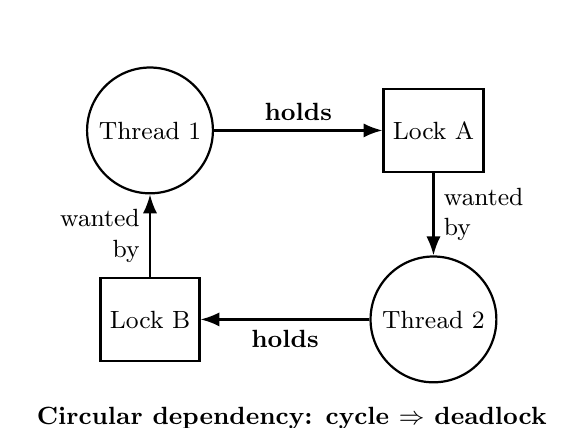
\begin{tikzpicture}[th/.style={circle, draw, thick, minimum size=1.35cm, font=\small},
                    lk/.style={rectangle, draw, thick, minimum size=1.05cm, font=\small},
                    >={Latex[length=2.4mm]}]
  \node[th] (t1) at (0,2.4) {Thread 1};
  \node[lk] (la) at (3.6,2.4) {Lock A};
  \node[lk] (lb) at (0,0) {Lock B};
  \node[th] (t2) at (3.6,0) {Thread 2};
  \draw[->, thick] (t1) -- node[above, font=\small\bfseries] {holds} (la);
  \draw[->, thick] (la) -- node[right, font=\small, align=left] {wanted\\by} (t2);
  \draw[->, thick] (t2) -- node[below, font=\small\bfseries] {holds} (lb);
  \draw[->, thick] (lb) -- node[left, font=\small, align=right] {wanted\\by} (t1);
  \node[font=\small\bfseries] at (1.8,-1.25) {Circular dependency: cycle $\Rightarrow$ deadlock};
\end{tikzpicture}
\end{center}

\subsection{Fix deadlocked code}

\begin{quizbox}[How would you fix this code?]
Make both threads acquire the locks in the \textbf{same order}:

\begin{center}
\begin{minipage}[t]{0.4\textwidth}
\textbf{Thread 1:}
\begin{lstlisting}[numbers=none]
lock(&A);
lock(&B);
\end{lstlisting}
\end{minipage}\hspace{2em}
\begin{minipage}[t]{0.4\textwidth}
\textbf{Thread 2:}
\begin{lstlisting}[numbers=none]
lock(&A);
lock(&B);
\end{lstlisting}
\end{minipage}
\end{center}
\end{quizbox}

Now whoever gets \texttt{A} first will also be able to get \texttt{B}; the
other thread waits for \texttt{A} while holding \emph{nothing}. The graph has
no cycle: \textbf{non-circular dependency (fine)}.

\begin{center}
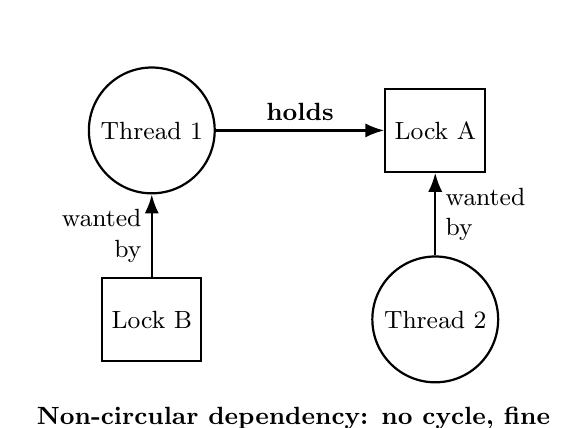
\begin{tikzpicture}[th/.style={circle, draw, thick, minimum size=1.35cm, font=\small},
                    lk/.style={rectangle, draw, thick, minimum size=1.05cm, font=\small},
                    >={Latex[length=2.4mm]}]
  \node[th] (t1) at (0,2.4) {Thread 1};
  \node[lk] (la) at (3.6,2.4) {Lock A};
  \node[lk] (lb) at (0,0) {Lock B};
  \node[th] (t2) at (3.6,0) {Thread 2};
  \draw[->, thick] (t1) -- node[above, font=\small\bfseries] {holds} (la);
  \draw[->, thick] (t2) -- node[right, font=\small, align=left] {wanted\\by} (la);
  \draw[->, thick] (lb) -- node[left, font=\small, align=right] {wanted\\by} (t1);
  \node[font=\small\bfseries] at (1.8,-1.25) {Non-circular dependency: no cycle, fine};
\end{tikzpicture}
\end{center}

Thread 1 holds A and wants B (which is free, so it gets it); Thread 2 wants A
and holds nothing. Thread 2 simply waits until Thread 1 is done. (On this
slide the Thread 2 edge is drawn upward into Lock A; it still means
``Lock A is wanted by Thread 2''.)

\keepspace{15\baselineskip}
\subsection{What's wrong? Encapsulation hides deadlocks}

\begin{lstlisting}
set_t *set_intersection (set_t *s1, set_t *s2) {
    set_t *rv = Malloc(sizeof(*rv));
    Mutex_lock(&s1->lock);
    Mutex_lock(&s2->lock);
    for(int i=0; i<s1->len; i++) {
        if(set_contains(s2, s1->items[i]))
            set_add(rv, s1->items[i]);
    }
    Mutex_unlock(&s2->lock);
    Mutex_unlock(&s1->lock);
    return rv;
}
\end{lstlisting}
{\small (The slide's code is missing a \texttt{)}, the \texttt{for} loop's
\texttt{\}} and \texttt{return rv;}; these are fixed here. They are not the
point of the question.)}

\medskip
\noindent\textbf{Encapsulation: modularity can make it harder to see
deadlocks.} The function always locks its \emph{first argument} first. Two
callers who pass the same sets in opposite orders get the circular-wait
example from before, hidden inside a library call:

\begin{center}
\begin{minipage}[t]{0.44\textwidth}
\textbf{Thread 1:}
\begin{lstlisting}[numbers=none]
rv = set_intersection(setA, setB);
\end{lstlisting}
\end{minipage}\hfill
\begin{minipage}[t]{0.44\textwidth}
\textbf{Thread 2:}
\begin{lstlisting}[numbers=none]
rv = set_intersection(setB, setA);
\end{lstlisting}
\end{minipage}
\end{center}
Thread 1 locks \texttt{setA->lock} and then wants \texttt{setB->lock}; Thread
2 locks \texttt{setB->lock} and then wants \texttt{setA->lock}. Neither caller
can see this from the function's interface.

\keepspace{22\baselineskip}
\begin{solbox}[Solution?]
Inside the function, acquire the two locks in a fixed \textbf{global} order
that does not depend on the argument order, e.g.\ by lock \textbf{address}
(with \texttt{m1}, \texttt{m2} being pointers to the two mutexes):
\begin{lstlisting}[numbers=none]
if (m1 > m2) {
    // grab locks in high-to-low address order
    pthread_mutex_lock(m1);
    pthread_mutex_lock(m2);
} else {
    pthread_mutex_lock(m2);
    pthread_mutex_lock(m1);
}
\end{lstlisting}
Both \texttt{set\_intersection(setA, setB)} and
\texttt{set\_intersection(setB, setA)} now lock the same mutex first, so no
cycle can form.

\textbf{Any other problems?} The code \textbf{assumes \texttt{m1 != m2}}
(not the same lock). If a caller does \texttt{set\_intersection(setA, setA)},
then \texttt{m1 == m2}, the \texttt{else} branch locks the same mutex twice,
and the thread deadlocks on itself. That case must be handled separately
(lock only once).
\end{solbox}

\keepspace{16\baselineskip}
% ===========================================================================
\section{Deadlock theory: the four conditions}
% ===========================================================================

\begin{keybox}[Conditions for deadlock]
Four conditions need to hold for a deadlock to occur.

\smallskip
\renewcommand{\arraystretch}{1.25}
\begin{tabularx}{\linewidth}{@{}lX@{}}
  \toprule
  \textbf{Condition} & \textbf{Description} \\
  \midrule
  Mutual exclusion & Threads claim exclusive control of resources that they require. \\
  Hold-and-wait & Threads hold resources allocated to them while waiting for additional resources. \\
  No preemption & Resources cannot be forcibly removed from threads that are holding them. \\
  Circular wait & There exists a circular chain of threads such that each thread holds one or more resources that are being requested by the next thread in the chain. \\
  \bottomrule
\end{tabularx}

\smallskip
If any of these four conditions are not met, \textbf{deadlock cannot occur}.
\end{keybox}

In the four-car intersection: each car has the part of the road it is on to
itself (\emph{mutual exclusion}); it keeps that part while waiting for the
part in front (\emph{hold-and-wait}); no car can be pushed back
(\emph{no preemption}); and A waits for B, B for D, D for C, C for A
(\emph{circular wait}).

\begin{keybox}[Deadlock theory]
Deadlocks can only happen with these \textbf{four} conditions: mutual
exclusion, hold-and-wait, no preemption, circular wait.

\textbf{Eliminate deadlock by eliminating any one condition.}
\end{keybox}

\keepspace{10\baselineskip}
The rest of the lecture takes the conditions one at a time:

\begin{center}
\renewcommand{\arraystretch}{1.2}
\begin{tabularx}{\textwidth}{@{}llX@{}}
  \toprule
  \textbf{Condition removed} & \textbf{Strategy} & \textbf{Main cost} \\
  \midrule
  Mutual exclusion & wait-free algorithms (compare-and-swap) & hard to design beyond simple structures \\
  Hold-and-wait & acquire all locks atomically (meta lock) & must know locks in advance; one big lock \\
  No preemption & \texttt{trylock()}, release what you hold & livelock (fix: exponential back-off) \\
  Circular wait & global order on lock acquisition & must be documented and followed everywhere \\
  \bottomrule
\end{tabularx}
\end{center}

\keepspace{12\baselineskip}
% ===========================================================================
\section{Eliminating mutual exclusion: wait-free algorithms}
% ===========================================================================

\begin{defbox}[Mutual exclusion]
Threads claim exclusive control of resources that they require (e.g., a
thread grabs a lock).
\end{defbox}

\textbf{Strategy: eliminate locks!} Try to replace locks with an atomic
hardware primitive:

\begin{lstlisting}[numbers=none]
int CompAndSwap(int *addr, int expected, int new)
// Returns 0: fail, 1: success
\end{lstlisting}
As in the locks lecture, \texttt{CompAndSwap} atomically checks whether
\texttt{*addr == expected}; if so it writes \texttt{new} into \texttt{*addr}
and returns 1, otherwise it changes nothing and returns 0.

\subsection{Atomic add}

\begin{center}
\begin{minipage}[t]{0.4\textwidth}
\textbf{With a lock:}
\begin{lstlisting}[numbers=none]
void add (int *val, int amt) {
    Mutex_lock(&m);
    *val += amt;
    Mutex_unlock(&m);
}
\end{lstlisting}
\end{minipage}\hfill
\begin{minipage}[t]{0.54\textwidth}
\textbf{Wait-free:}
\begin{lstlisting}[numbers=none]
void add (int *val, int amt) {
    int old;
    do {
        old = *val;
    } while (!CompAndSwap(val, ??, old+amt));
}
\end{lstlisting}
\end{minipage}
\end{center}
{\small (The slide writes \texttt{*value}, leaves out the last \texttt{)}, and
declares \texttt{int old} inside the loop body, where the \texttt{while}
condition cannot see it; all three are fixed here.)}

\begin{quizbox}[What goes in place of \texttt{??}]
\texttt{??} \(=\) \texttt{old}:
\texttt{while (!CompAndSwap(val, old, old+amt));}

Read the current value into \texttt{old}, then try to replace it with
\texttt{old+amt}, but \emph{only if it is still} \texttt{old}. If another
thread changed \texttt{*val} in between, the CAS fails (returns 0) and we
retry with the new value. No lock is ever held, so no deadlock is possible.
Strictly speaking these CAS retry loops are lock-free rather than wait-free:
no thread ever blocks, but one thread can in principle keep failing its CAS
while others succeed.
\end{quizbox}

\keepspace{14\baselineskip}
\subsection{Linked list insert}

\begin{center}
\begin{minipage}[t]{0.46\textwidth}
\textbf{With a lock:}
\begin{lstlisting}[numbers=none]
void insert (int val) {
    node_t *n = Malloc(sizeof(*n));
    n->val = val;
    lock(&m);
    n->next = head;
    head = n;
    unlock(&m);
}
\end{lstlisting}
\end{minipage}\hfill
\begin{minipage}[t]{0.51\textwidth}
\textbf{Wait-free:}
\begin{lstlisting}[numbers=none]
void insert (int val) {
    node_t *n = Malloc(sizeof(*n));
    n->val = val;
    do {
        n->next = head;
    } while (!CompAndSwap(  ??  ));
}
\end{lstlisting}
\end{minipage}
\end{center}

Without any synchronization, two threads inserting at once can both read the
same \texttt{head}, both point their new node at it, and both write
\texttt{head}; one of the two nodes is then lost. The locked version prevents
this by making lines \texttt{n->next = head; head = n;} a critical section.
Allocation and filling in \texttt{n->val} touch only the new, private node,
so they stay outside the lock.

\begin{solbox}[Filling in the CAS]
\begin{lstlisting}[numbers=none]
void insert (int val) {
    node_t *n = Malloc(sizeof(*n));
    n->val = val;
    do {
        n->next = head;
    } while (!CompAndSwap(&head, n->next, n));
}
\end{lstlisting}
Point the new node at the current head, then swing \texttt{head} to the new
node \emph{only if} \texttt{head} still equals the value we read
(\texttt{n->next}). If another thread inserted in the meantime,
\texttt{head} has changed, the CAS fails, and we loop: re-read
\texttt{head}, re-link, and try again. (Here CAS is applied to pointers
rather than \texttt{int}s; it is the same atomic compare-and-swap on one
machine word.)
\end{solbox}

\keepspace{12\baselineskip}
% ===========================================================================
\section{Eliminating hold-and-wait}
% ===========================================================================

\begin{defbox}[Hold-and-wait]
Threads hold resources allocated to them (e.g., locks they have already
acquired) while waiting for additional resources (e.g., locks they wish to
acquire).
\end{defbox}

\textbf{Strategy: acquire all locks atomically \emph{once}.} A thread can
release locks over time, but cannot acquire again until all have been
released.

\textbf{How to do this?} Use a \textbf{meta lock}, like this:

\begin{lstlisting}
lock(&meta);
lock(&L1);
lock(&L2);
...
unlock(&meta);

// Critical section code

unlock(...);
\end{lstlisting}

Because every thread must hold \texttt{meta} while it acquires its locks, no
other thread can grab a lock part-way through. So a thread is never stuck
holding some of its locks while another thread holds the rest.

\begin{warnbox}[Disadvantages?]
\begin{itemize}
  \item Must know \textbf{ahead of time} which locks will be needed.
  \item Must be \textbf{conservative} (acquire any lock possibly needed).
  \item \textbf{Degenerates to just having one big lock}: locks are taken
        early and held long, so concurrency drops.
\end{itemize}
\end{warnbox}

\keepspace{12\baselineskip}
% ===========================================================================
\section{Eliminating no preemption}
% ===========================================================================

\begin{defbox}[No preemption]
Resources (e.g., locks) cannot be forcibly removed from threads that are
holding them.
\end{defbox}

\textbf{Strategy: support preemption.} If a thread can't get what it wants,
it \textbf{releases what it holds}. This uses \texttt{trylock(B)}, which
acquires \texttt{B} if it is free and otherwise returns \(-1\) at once
instead of waiting.

\begin{lstlisting}
top:
    lock(A);
    if (trylock(B) == -1) {
        unlock(A);
        goto top;
    }
    ...
\end{lstlisting}

The thread never waits for \texttt{B} while holding \texttt{A}. Even if
another thread follows the same pattern with the locks in the opposite order,
neither can block the other forever.

\begin{warnbox}[Disadvantages?]
\textbf{Livelock:} no processes make progress, but the state of the involved
processes constantly changes. For example, two threads repeatedly grab their
first lock, fail the \texttt{trylock}, release, jump to \texttt{top}, and
collide again, over and over. They are not blocked (so this is not deadlock),
but neither gets anything done.

\textbf{Classic solution: exponential back-off.} After each failure, wait a
random delay before retrying, doubling the maximum delay each time, so the
threads stop colliding in step.
\end{warnbox}

\keepspace{12\baselineskip}
% ===========================================================================
\section{Eliminating circular wait}
% ===========================================================================

\begin{defbox}[Circular wait]
There exists a circular chain of threads such that each thread holds a
resource (e.g., lock) being requested by the next thread in the chain.
\end{defbox}

\begin{keybox}[Strategy]
\begin{itemize}
  \item Decide which locks should be acquired before others.
  \item If A before B, \textbf{never acquire A if B is already held!}
  \item Document this, and write code accordingly.
\end{itemize}
Works well if the system has \textbf{distinct layers}.
\end{keybox}

With a fixed order, every thread waits only for locks that come
\emph{later} in the order than the ones it holds, so the waiting chain can
never close into a cycle. The two fixes seen earlier are both this
strategy: in the code example, both threads take \texttt{A} before
\texttt{B}; in \texttt{set\_intersection}, the locks are taken in
high-to-low address order. It is only a convention, though: a single piece
of code that takes the locks in the wrong order can bring the deadlock back.

\keepspace{20\baselineskip}
% ===========================================================================
\section{Summary}
% ===========================================================================

\begin{keybox}[Concurrency bugs]
\begin{itemize}
  \item Concurrency bugs are real and can be deadly (Therac-25). In the Lu et
        al.\ study of MySQL, Apache, Mozilla and OpenOffice, most bugs were
        \textbf{atomicity}, \textbf{order} or \textbf{deadlock} bugs.
  \item \textbf{Atomicity bug:} code that should be atomic (check then use)
        is not. Fix with \textbf{locks} around every access to the shared
        data.
  \item \textbf{Ordering bug:} A must happen before B but this is not
        enforced. Fix with \textbf{condition variables} (state variable +
        \texttt{while} + \texttt{wait}/\texttt{signal}).
  \item \textbf{Deadlock:} threads wait for each other forever (``deadly
        embrace''). It shows up as a \textbf{cycle} in the dependency graph
        and may happen only on some interleavings. Encapsulation can hide it
        (e.g.\ \texttt{set\_intersection(setA, setB)} versus
        \texttt{set\_intersection(setB, setA)}).
  \item Deadlock needs all four of: \textbf{mutual exclusion,
        hold-and-wait, no preemption, circular wait}. Remove any one:
    \begin{itemize}
      \item mutual exclusion \(\to\) wait-free code with
            \texttt{CompAndSwap};
      \item hold-and-wait \(\to\) grab all locks atomically under a meta
            lock;
      \item no preemption \(\to\) \texttt{trylock}, release and retry (watch
            for livelock; use exponential back-off);
      \item circular wait \(\to\) a global lock order (e.g.\ by address),
            documented and followed.
    \end{itemize}
\end{itemize}
\end{keybox}

\end{document}
